\chapter{Anhang}
\label{ch:anhang}

\section{Liste der gesichteten Urkunden des \citetitle{cao}}
\label{sec:urkliste}

Die folgenden zwei Listen enthalten die Urkundennummern im \citetitle{cao}, die
für die Auswertung gesichtet wurden, mit ihren IDs in \citet{cao-online}.%
%
	\footnote{Um zum jeweiligen Text zu gelangen, ist die angegebene ID der
	folgenden URL nachzustellen:
	\url{http://tcdh01.uni-trier.de/cgi-bin/iCorpus/CorpusIndex.tcl?for=qfcoraltdu&cnt=qfcoraltdu&xid=}\textsc{<id>}.}
%
Dabei sind nicht alle Urkunden in die Auswertung eingeflossen. Überschneidungen
mit dem \citet{rem} und der Stichprobe der \tit{Mittelhochdeutschen Grammatik}
von \citet{ksw3,ksw2} sind in der Spalte \q*{ReM} markiert. Sofern eine
Abbildung der betreffenden Urkundennummer öffentlich verfügbar im Internet
gefunden werden konnte (Stand: \DTMdate{2022-02-20}), wird deren URL angegeben.%
%
	\footnote{Wo keine vollständige URL angegeben ist, ist der angegebene
	Pfad der folgenden URL nachzustellen:
	\url{https://www.monasterium.net/mom/}\textsc{<pfad>}.}

\subsection{Ausgewertete Urkunden}
\label{subsec:ausgewurk}

\begin{xltabular}{\linewidth}{@{} l c l X @{}}
\toprule
\textbf{Nr.}
	& \textbf{ReM}
	& \textbf{CAO Online}
	& \textbf{Abbildung}
	\\
\midrule
\endfirsthead

\textbf{Nr.}
	& \textbf{ReM}
	& \textbf{CAO Online}
	& \textbf{Abbildung}
	\\
\midrule
\endhead

\bottomrule
\endlastfoot

31		&           & CW10038 \\
75		& $\bullet$ & CW10087 \\
76		& $\bullet$ & CW10088 \\
81		&           & CW10093 \\
85		& $\bullet$ & CW10097 \\
86		&           & CW10098 \\
165		&           & CW10182 \\
171		&           & CW10189 \\
179		&           & CW10197 \\
190		&           & CW10209 \\
199		&           & CW10218 \\
201		&           & CW10220 \\
214		&           & CW10233 \\
260		&           & CW10284 \\
326		&           & CW10358 \\
371		&           & CW10405 \\
389		&           & CW10423 \\
415		&           & CW10451 \\
429		& $\bullet$ & CW10465 \\
491		&           & CW10529
		& \url{AT-HHStA/SbgDK/AUR_1281_XII_07/charter}
	\\
508		& $\bullet$ & CW10549 \\
519		&           & CW10560 \\
524		&           & CW10565 \\
560		& $\bullet$ & CW10609 \\
583		&           & CW20022 \\
604		&           & CW20043
		& \url{DE-StaAWo/Abt1AI/I-0063/charter}
	\\
610		&           & CW20049 \\
619		&           & CW20059 \\
627		&           & CW20067 \\
629		&           & CW20069 \\
632		&           & CW20072 \\
636		&           & CW20076
		& \url{AT-StiAStams/Urkunden/A_XLII_1/charter}
	\\
656		&           & CW20097 \\
682		&           & CW20126 \\
701		&           & CW20145 \\
923		&           & CW20381
		& \url{DE-BayHStA/KUAldersbach/00093/charter}
	\\
925		&           & CW20383 \\
937		&           & CW20395 \\
971~A, B	&           & CW20431, CW20432 \\
1001	&           & CW20463 \\
1055	&           & CW20521 \\
1073	&           & CW20539
		& \url{AT-StiAH/WienOCist/1289/charter}
	\\
1121	&           & CW20591 \\
1126~A, B	&           & CW20596, CW20597 \\
1137	&           & CW20608
		& \url{AT-StiAH/WienOCist/1289/charter}
	\\
1153	&           & CW20627 \\
1154	&           & CW20628 \\
1201~A, B	&           & CW20677, CW20678 \\
1217	&           & CW20694
		& \url{AT-HHStA/SbgDK/AUR_1290_III_12/charter}
	\\
1218	&           & CW20695 \\
1221	&           & CW20698 \\
1229	&           & CW20706
		& \url{AT-StiAFiecht/Urkunden/U107/charter}
	\\
1234	&           & CW20711 \\
1259	&           & CW20736 \\
1270	&           & CW20748 \\
1282	&           & CW20763 \\
1352	&           & CW20838 \\
1359	&           & CW20846 \\
1382	&           & CW20870
		& \url{AT-StiALi/LilienfeldOCist/1291_III_11/charter}
	\\
1414	&           & CW20903 \\
1416	&           & CW20905 \\
1436	&           & CW20927
		& \url{AT-HHStA/SbgDK/AUR_1291_VI_15/charter}
	\\
1503	&           & CW20997 \\
1504	&           & CW20998 \\
1514	&           & CW21008 \\
1545	&           & CW21039 \\
1566	&           & CW21061 \\
1568	&           & CW21063
		& \url{AT-StiAH/HeiligenkreuzOCist/1292_IV_21/charter}
	\\
1578	&           & CW21073
		& \url{AT-DOZA/Urkunden/1027/charter}
	\\
1584	&           & CW21079 \\
1620	&           & CW21118 \\
1657	&           & CW21157
		& \url{DE-BayHStA/HUPassau/250/charter}
	\\
1661	&           & CW30004 \\
1747	&           & CW30091 \\
1764	&           & CW30108 \\
1802	&           & CW30149
		& \url{CH-StiASG/Urkunden/PPP.4_Nr_1/charter}
	\\
1831	&           & CW30178
		& \url{DE-StaAWo/Abt1AI/I-0077/charter}
	\\
1843	&           & CW30190 \\
1898	&           & CW30246 \\
1950	&           & CW30300 \\
1956	&           & CW30306
		& \url{CH-StiASG/Urkunden/CC.4.E.1/charter}
	\\
1971	&           & CW30321 \\
1972~A, B	&           & CW30322, CW30323 \\
2001	& $\bullet$ & CW30353 \\
2011	&           & CW30363
		& \url{AT-StiASei/SeitenstettenOSB/1294_VIII_24/charter}
	\\
2055	&           & CW30363 \\
2092	&           & CW30445 \\
2110	&           & CW30463
		& \url{DE-BayHStA/KUAldersbach/00133/charter}
	\\
2174	&           & CW30529 \\
2183	&           & CW30538 \\
2214	&           & CW30569 \\
2240	&           & CW30597 \\
2253	&           & CW30611
		& \url{AT-OOeLA/GarstenOSB/1295_X_10/charter}
	\\
2293	&           & CW30652 \\
2307	&           & CW30666
		& \url{DE-BayHStA/KUMuenchenAngerkloster/32/charter}
	\\
2309	&           & CW30668
		& \url{http://www.landesarchiv-bw.de/plink/?f=2-5271672}
	\\
2310	&           & CW30669 \\
2338~A, B	&            & CW30698, CW30699 \\
2350	&           & CW30711 \\
2353	&           & CW30714 \\
2359	&           & CW30720 \\
2367	&           & CW30728 \\
2375	&           & CW30736 \\
2396	&           & CW30757 \\
2401	&           & CW30762 \\
2406	&           & CW30767 \\
2412	&           & CW30773
		& \url{AT-StiAK/KlosterneuburgCanReg/1296_V_01/charter}
	\\
2445	&           & CW30807 \\
2468	&           & CW30831 \\
2497	&           & CW30860 \\
2532	&           & CW30896 \\
2535	&           & CW30899 \\
2563	&           & CW40004 \\
2568	&           & CW40009 \\
2583	&           & CW40025 \\
2625~A, B	&           & CW40067, CW40068 \\
2651~A, B	&           & CW40094, CW40095 \\
2694	&           & CW40139
		& \url{AT-StiASF/StFlorianCanReg/1297_IV_24/charter}
	\\
2713	&           & CW40158 \\
2719	&           & CW40164 \\
2733	& $\bullet$ & CW40179 \\
2735~A, B	&           & CW40181, CW40182 \\
2748	&           & CW40196 \\
2824	&           & CW40275 \\
2843	&           & CW40295
		& \url{AT-HHStA/SbgE/AUR_1297_XI_20/charter}
	\\
2862	&           & CW40315 \\
2866	&           & CW40319 \\
2872	&           & CW40325 \\
2913	&           & CW40366 \\
2915	&           & CW40368 \\
2925	&           & CW40378 \\
2930	&           & CW40383 \\
2931	&           & CW10318 \\
2957	&           & CW40410 \\
2960	&           & CW40413 \\
2962	&           & CW40415
		& \url{AT-OOeLA/GarstenOSB/1298_IV_06/charter}
	\\
3020~A, B	&           & CW40476, CW40477
	& \makecell[tl]{\url{AT-OOeLA/GarstenOSB/1298_VI/charter}\\
		(A~=~Bl.~88r, B~=~Bl.~86r)}
	\\
3022	&           & CW40479 \\
3034	&           & CW40491 \\
3038	&           & CW40495 \\
3049	&           & CW40506 \\
3056	&           & CW40515 \\
3062	&           & CW40521
		& \url{AT-StiAZ/Urkunden/1298_IX_01/charter}
	\\
3104	&           & CW40563 \\
3116	&           & CW40575 \\
3130	&           & CW40589 \\
3133	&           & CW40592 \\
3141~A, B	&           & CW40600, CW40601 \\
3147	&           & CW40607 \\
3150	&           & CW40610 \\
3160	&           & CW40620 \\
3171	&           & CW40632 \\
3224~A, B	&           & CW40685, CW40686 \\
3249	&           & CW40712 \\
3261	&           & CW40725 \\
3262	&           & CW40726 \\
3319	&           & CW40785 \\
3330	&           & CW40796 \\
3331	&           & CW40797 \\
3332	&           & CW40798 \\
3339	&           & CW40805 \\
3346	&           & CW40812 \\
3376	&           & CW40842 \\
3397	&           & CW40863 \\
3428	&           & CW40897 \\
3451	&           & CW40920 \\
3536	&           & CW41005
		& \url{AT-HHStA/SbgDK/AUR_1299_XI_28/charter}
	\\
N~2~A, B	&           & CW50002, CW50003 \\
N~11	&           & CW50013 \\
N~14	&           & CW50016 \\
N~52	&           & CW50054 \\
N~92	&           & CW50094 \\
N~99	&           & CW50101 \\
N~109~A, B	&           & CW50111, CW50112 \\
N~150	&           & CW50155 \\
N~197	&           & CW50206 \\
N~202	&           & CW50211 \\
N~210	&           & CW50219 \\
N~220	&           & CW50229 \\
N~230	&           & CW50239 \\
N~235	&           & CW50244 \\
N~272	& $\bullet$ & CW50282 \\
N~288	&           & CW50298 \\
N~294	&           & CW50304 \\
N~305	&           & CW50315 \\
N~321	&           & CW50331 \\
N~328	&           & CW50340 \\
N~357	&           & CW50370 \\
N~377	&           & CW50391 \\
N~384	&           & CW50398 \\
N~385	&           & CW50399 \\
N~386	&           & CW50400
		& \url{AT-HKA/Urkunden/1289/charter}
	\\
N~401	&           & CW50415 \\
N~456	&           & CW50470 \\
N~463	&           & CW50477 \\
N~475	&           & CW50489
	& \url{AT-HHStA/TullnOP/1291/charter}
	\\
N~518	&           & CW50534
	& \url{AT-NOeLA/StA_Urk/StA_Urk_0024/charter}
	\\
N~524	&           & CW50540 \\
N~557	&           & CW50575
		& \url{AT-WStLA/HAUrk/21/charter}
	\\
N~590	&           & CW50608
		& \url{AT-WStLA/HA, Bsp/9/charter}
	\\
N~689	&           & CW50710 \\
N~701	&           & CW50722 \\
N~709	&           & CW50730 \\
N~723	&           & CW50745 \\
N~727	&           & CW50749 \\
N~748	&           & CW50770.1 \\
N~752	&           & CW50774 \\
N~756	&           & CW50778 \\
N~766	&           & CW50788 \\
N~812	&           & CW50835 \\
\end{xltabular}

\subsection{Ausgesonderte Urkunden}
\label{subsec:ausgesurk}

Neben solchen Urkunden, die im Ortsregister von \citet{cao-online} mehreren
Ausstellungsorten zugewiesen sind und/oder deren Ausstellungsjahr nicht
eindeutig feststellbar ist, wurden die im Folgenden aufgelisteten Urkunden
zusätzlich nicht in die Auswertung aufgenommen.

\begin{xltabular}{\linewidth}{@{} l c l X @{}}
\toprule
\textbf{Nr.}
	& \textbf{ReM}
	& \textbf{CAO Online}
	& \textbf{Abbildung}
	\\
\midrule
\endfirsthead

\textbf{Nr.}
	& \textbf{ReM}
	& \textbf{CAO Online}
	& \textbf{Abbildung}
	\\
\midrule
\endhead

\bottomrule
\endlastfoot

69 A	&           & CW10079 \\
71		&           & CW10082 \\
72 B	& $\bullet$ & CW10084 \\
78		& $\bullet$ & CW10090 \\
83		& $\bullet$ & CW10095 \\
131		&           & CW10146 \\
190		&           & CW10209 \\
369		&           & CW10403 \\
491		&           & CW10529
		& \url{AT-HHStA/SbgDK/AUR_1281_XII_07/charter}
	\\
501 A, B	&           & CW10541, CW10542 \\
508		& $\bullet$ & CW10549 \\
549		& $\bullet$ & CW10597 \\
559		&           & CW10608 \\
602		&           & CW20041 \\
623		&           & CW20063 \\
661 A, B	&           & CW20102, CW20103 \\
677		& $\bullet$ & CW20120 \\
777		&           & CW20223 \\
885		&           & CW20341 \\
904		&           & CW20360 \\
979		&           & CW20440 \\
1076	&           & CW20542 \\
1145	&           & CW20618 \\
1169	&           & CW20644 \\
1234	&           & CW20711 \\
1304	&           & CW20786 \\
1429	&           & CW20918
		& \url{AT-HHStA/SbgE/AUR_1291_VI_07/charter}
	\\
1460	&           & CW20953 \\
1662	&           & CW30005
		& \url{http://www.landesarchiv-bw.de/plink/?f=2-2372216}.
	\\
1717	&           & CW30060 \\
1758	&           & CW30102 \\
1820	&           & CW30167 \\
1923	&           & CW30272
		& \url{AT-HHStA/SbgE/AUR_1294_III_18/charter}
	\\
2005	&           & CW30357 \\
2008	& $\bullet$ & CW30360 \\
2033	&           & CW30385 \\
2111	&           & CW30464
		& \url{DE-BayHStA/KUNiederaltaich/107/charter}
	\\
2226	&           & CW30581 \\
2366	&           & CW30727 \\
2520	&           & CW30884 \\
2522	&           & CW30886 \\
2529	&           & CW30893 \\
2607	&           & CW40049 \\
2694	&           & CW40139
	& \url{AT-StiASF/StFlorianCanReg/1297_IV_24/charter}
	\\
2748	&           & CW40196 \\
2786	&           & CW40235 \\
2841	&           & CW40293 \\
3045	&           & CW40502 \\
3047	&           & CW40504 \\
3248	&           & CW40711 \\
3330	&           & CW40796 \\
3376	&           & CW40842 \\
3496	&           & CW40965 \\
N 36	& $\bullet$ & CW50038 \\
N 68	& $\bullet$ & CW50070 \\
N 100	&           & CW50102 \\
N 115	&           & CW50118 \\
N 235	&           & CW50244 \\
N 241	&           & CW50251 \\
N 294	&           & CW50304 \\
N 305	&           & CW50315 \\
N 337	&           & CW50350 \\
N 524	&           & CW50540 \\
N 526	&           & CW50542 \\
N 567	&           & CW50585 \\
N 664	&           & CW50685 \\
N 674	&           & CW50695 \\
N 702	&           & CW50723
		& \url{AT-NOeLA/StA_Urk/StA_Urk_0027/charter}
	\\

\end{xltabular}

\section{Stichprobe zur Grafie von mhd.\ \norm{e}}
\label{sec:caoalemschwa}

Die Schreibweise \lit{i} für den unbetonten Nebensilbenvokal mhd.~\norm{e} [ə]
gilt unter den ober\-deutschen Schreibdialekten als alemannisches Kennzeichen
\autocites[vgl.][25]{weinhold1863}[75]{weinhold1883}[41, 113]{paul2007}, jedoch
findet sich \lit{-i} in der Stichprobe zu \norm{bėide} \wdef{beide}
typischerweise in solchen Kontexten, in denen ursprünglich \norm{-iu} /yː/
vorlag (siehe \cref{fn:caoalemschwa,subsec:cao_adjflex_disc}). Um
sicherzustellen, dass \lit{-i} in alemannischen Urkunden tatsächlich die
ebenfalls für diese Region typische Entrundung von \norm{-iu} darstellt und
nicht etwa regelmäßig auch an anderen Stellen für einen unbetonten Vokal steht
\autocites%
	[466--467]{schirmunski1962}%
	[41]{paul2007}%
	[305]{ksw2}%
	[vgl.~auch][131--132]{boesch1946}%
, wurde eine gesonderte Teilauswertung auf Basis einer Stichprobe vorgenommen,
bei der die Grafie des Schwa-Lauts überprüft wurde.

Hierzu wurden die in \cref{tab:caoalemschwa} aufgeführten Lemmata für die
Ausstellungsorte
Straßburg (2.600 Belege),
% 	āne		 254
% 	hērre	1832
% 	hȫrent	  27
% 	umbe	 367
% 	vrouwe	 120
% 	Summe	2600
% 
Zürich (1.695),
% 	āne		  63
% 	hērre	1121
% 	hȫrent	 144
% 	umbe	 254
% 	vrouwe	 113
% 	Summe	1695
% 
Freiburg i.\,Br. (1.478),
% 	āne		  95
% 	hērre	 865
% 	hȫrent	 160
% 	umbe	 226
% 	vrouwe	 132
% 	Summe	1478
% 
Basel (1.028),
% 	āne		  32
% 	hērre	 532
% 	hȫrent	 126
% 	umbe	 194
% 	vrouwe	 144
% 	Summe	1028
% 
Colmar (849),
% 	āne		 60
% 	hērre	393
% 	hȫrent	 93
% 	umbe	184
% 	vrouwe	119
% 	Summe	849
% 
Konstanz (1.110),
% 	āne		 110
% 	hērre	 657
% 	hȫrent	  93
% 	umbe	 207
% 	vrouwe	  43
% 	Summe	1110
% 
Luzern (236),
% 	āne		  8
% 	hērre	142
% 	hȫrent	 21
% 	umbe	 37
% 	vrouwe	 28
% 	Summe	236
% 
Bern (35)
% 	āne		 2
% 	hērre	13
% 	hȫrent	 6
% 	umbe	14
% 	vrouwe	 0
% 	Summe	35
% 
und Chur (45)
% 	āne		 2
% 	hērre	30
% 	hȫrent	 4
% 	umbe	 9
% 	vrouwe	 0
% 	Summe	45
% 
basierend auf der automatischen Annotation der Lemmata nach dem Modell von
\citet{schmid2019} abgefragt. Wie in \cref{subsec:cao_sample} im Rahmen des
Aufbaus der Stichprobe zur Adjektivdeklination im \citetitle{cao} beschrieben,
wurden auch hier jeweils die Ausstellungsorte im Umkreis von etwa vierzig
Kilometern (0,25°) hinzugenommen. Die Lemmata wurden so ausgewählt, dass jeder
im Ahd.\ volle Nebensilbenvokal zumindest in der Zitationsform vorkommt und die
Lemmata möglichst häufig im \citetitle{cao} belegt sind. Bei der Abfrage wurden
nur solche Lemmata gewertet, deren Zuweisung und Formenbestimmung vom
Annotations\-algorithmus mit mindestens 95\pct{} Konfidenz bewertet wurde.

\begin{table}
\centering
\caption{Lemmata bzw. Wortformen der Stichprobe zur Grafie von Schwa}
\begin{tabular}{l l l r r @{~} r l}
\toprule

\mr{2}{*}[-.5ex]{\textbf{Ahd.}}
	& \mr{2}{*}[-.5ex]{\textbf{Mhd.}}
	& \mr{2}{*}[-.5ex]{\textbf{Übersetzung}}
	& \mc{3}{c}{\textbf{Häufigkeit}}
	& \mr{2}{*}[-.5ex]{\textbf{Quelle}}
	\\

\cmidrule(lr){4-6}

%
	& %
	& %
	& \textbf{Stichprobe}
	& %
	& \textbf{\citetitle{cao}}
	& %
	\\

\midrule

\norm{hērro}
	& \norm{hērre}
	& \wdef{Herr}
	& 5.521
	& ca.
	& 17.700
	& \cite[834--837]{wmu1}
	\\

\midrule

\norm{umbi}
	& \norm{umbe}
	& \wdef{um}
	& 1.482
	& ca.
	& 5.500
	& \cite[1857--1860]{wmu3}
	\\

\midrule

\norm{frouwa}
	& \norm{vrouwe}
	& \wdef{(Edel-)Frau}
	& 688
	& ca.
	& 4.500
	& \cite[2261--2263]{wmu3}
	\\

\midrule

\norm{hōrėnt}
	& \norm{hȫrent}
	& \wdef{(sie) hören}
	& 660
	& \norm{hȫren}:
	& 4.370
	& \cite[882--883]{wmu2}
	\\

\midrule

\norm{ānu}
	& \norm{āne}
	& \wdef{ohne}
	& 621
	& %
	& 4.270
	& \cite[90--91]{wmu1}
	\\

\bottomrule
\end{tabular}
\label{tab:caoalemschwa}
\end{table}

Die Karte in \cref{fig:caoalemschwa} gibt einen Überblick über die geografische
Variation der Grafie des unbetonten Vokals in der Stichprobe. Gut zu sehen ist,
dass \norm{e} und die Syn- oder Apokope des Vokals -- wie beispielsweise bei
\lit{hern} \wdef{Herrn} und \lit{hoͤrnt} \wdef{hören (\Tpl.\Ind.\Prs)} sowie
\lit{fron} \wdef{Frau (\Obl.\Sg), Frauen} und \lit{vmb} \wdef{um} --
vorherrschen. Schreibungen mit anderen Vokalen kommen nur selten vor, zum
Beispiel \lit{herrun} \wdef{Herrn, Herren} oder \norm{frowan} \wdef{Frauen}
(ahd. \norm{frouwūn}). Darüber hinaus liegen noch einige Fälle von
\lit{frown} vor, bei denen der Nebensilbenvokal vermutlich synkopiert ist,
jedoch die Schreibung \lit{w} für \norm{wu} nicht strikt ausgeschlossen werden
kann \autocite[vgl.][142]{paul2007}. Ein großer prozentualer Anteil von Grafien
mit \norm{i} fällt besonders in St.~Gallen ins Auge.

\begin{figure}
\centering
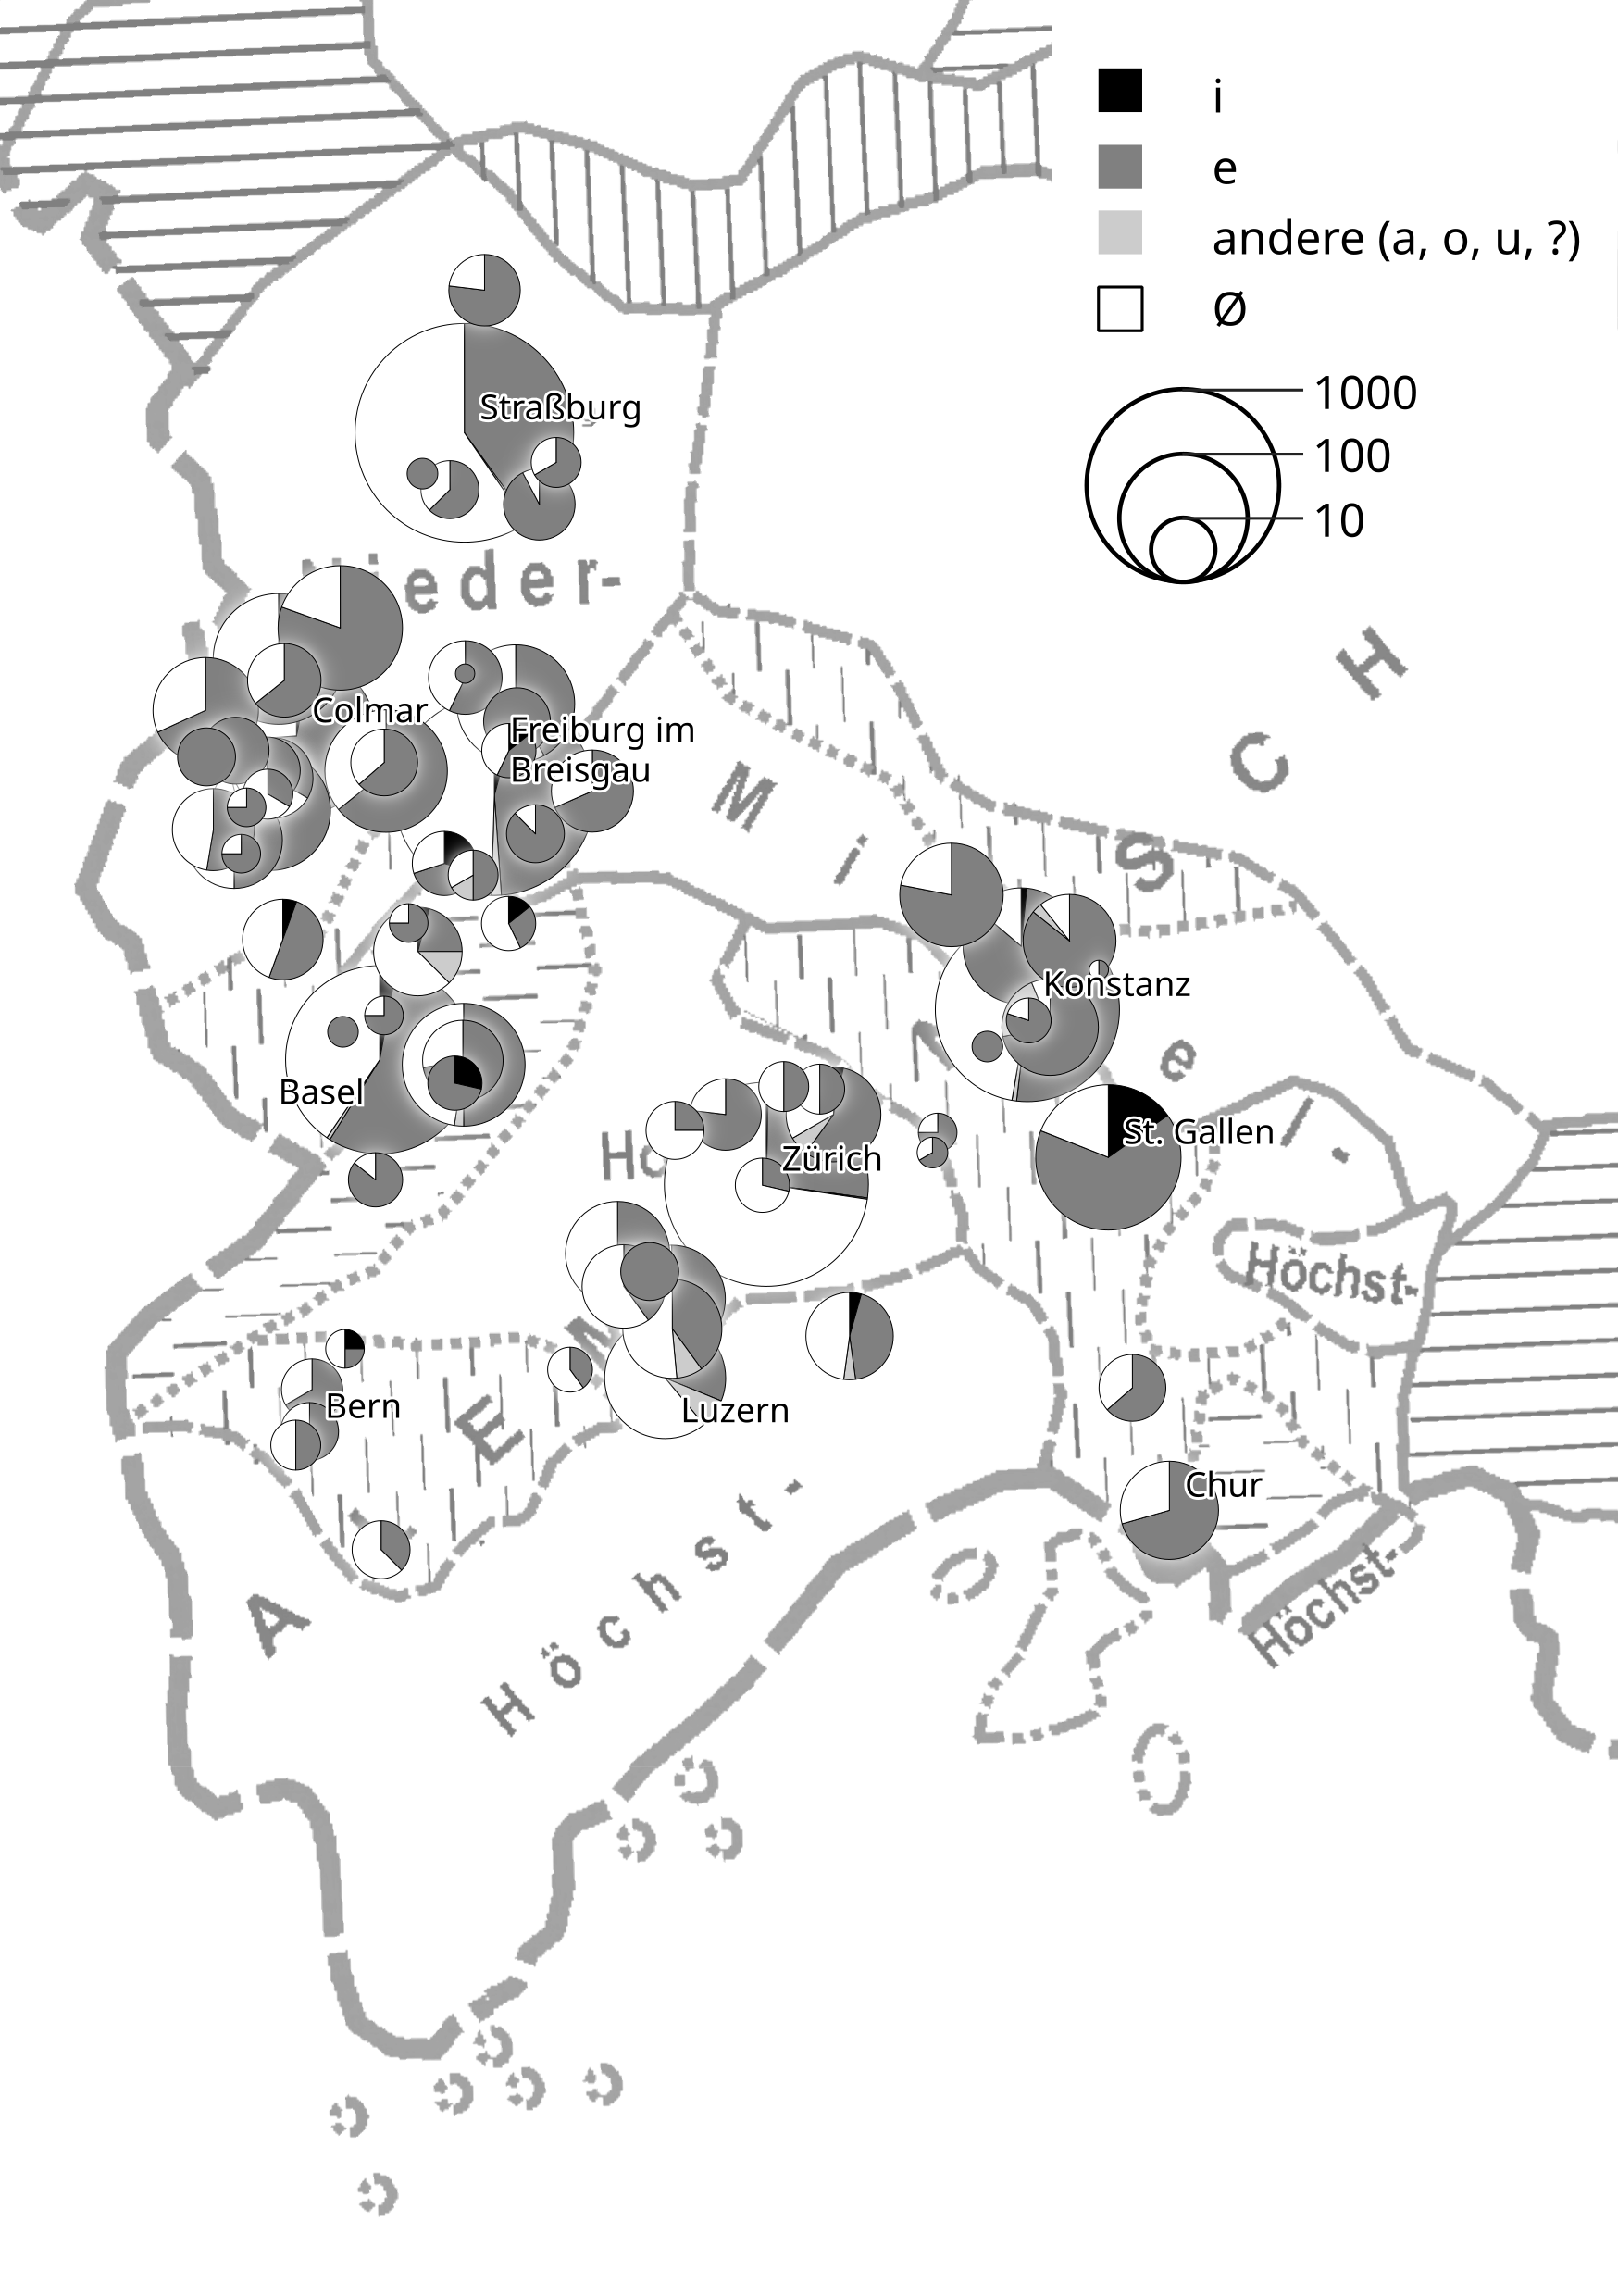
\includegraphics[
	height=.75\textheight,
	keepaspectratio
]{./assets/grafiken/2023-05-19_schwa_alem.png}
\caption{Geografische Verteilung der Stichprobe zur Grafie von Schwa\nocite{wiesinger1983:rede}}
\label{fig:caoalemschwa}
\end{figure}

In der Tat machen die 28 Belege aus St.~Gallen dort immerhin 15,2\pct{} der
belegten \lit{i}-Grafien aus, wie aus \cref{tab:ispelx} hervorgeht (diese zeigt
als Ausschnitt nur diejenigen Ausstellungsorte, an denen \norm{i}-Grafien
belegt sind). Hohe absolute Werte werden auch in Freiburg i.\,Br. (55 Belege)
sowie in Basel (25) und Konstanz (21) erreicht. Gemessen an der jeweiligen
Gesamtzahl der Belege pro Ausstellungsort machen sie allerdings nur einen
kleinen Teil aus (4,2\pct; 2,9\pct; 2,8\pct). An anderen Ausstellungsorten in
der Stichprobe kommen \norm{i}-Graphien nur vereinzelt vor.

\begin{table}
\centering
\caption{Anteil der \norm{i}-Grafie an betreffenden Schreiborten im Vergleich}
\begin{tabular}{
	l @{\qquad}
	r r @{\qquad}
	r r @{\qquad}
	r r @{\qquad}
	r r @{\qquad}
	r}

\toprule

\bfseries Ausstellungsort
	& \bfseries \norm{-i} & \bfseries \%
	& \bfseries \norm{-e} & \bfseries \%
	& \bfseries -Ø & \bfseries \%
	& \bfseries andere & \bfseries \%
	& \bfseries Summe
	\\

\midrule

Basel
	& 25	& 2,9
	& 481	& 56,0
	& 348	& 40,5
	& 5		& 0,6
	& 859
	\\

\midrule

Colmar
	& 10	& 3,2
	& 222	& 70,7
	& 82	& 26,1
	& 		&
	& 314
	\\

\midrule

Denzlingen
	& 1 & 14,3
	& 3	& 42,9
	& 3	& 42,9
	& 	&
	& 7
	\\

\midrule

Freiburg i.\,Br.
	& 55	& 4,2
	& 589	& 44,7
	& 652	& 49,5
	& 21	& 1,6
	& 1317
	\\

\midrule

Guebwiller
	& 1		& 3,1
	& 15	& 46,9
	& 16	& 50,0
	& 		&
	& 32
	\\

\midrule

Kl.~Einsiedeln
	& 1		& 4,3
	& 10	& 43,5
	& 11	& 47,8
	& 1		& 4,3
	& 23
	\\

\midrule

Kl.~Fraubrunnen
	& 1	& 25,0
	& 1	& 25,0
	& 2	& 50,0
	&	&
	& 4
	\\

\midrule

Kl.~Olsberg
	& 2	& 28,6
	& 5	& 71,4
	&	&
	&	&
	& 7
	\\

\midrule

Kl.~Sitzenkirch
	& 1		& 4,2
	& 5		& 20,8
	& 15	& 62,5
	& 3		& 12,5
	& 24
	\\

\midrule

Kl.~Töss
	& 1		& 3,3
	& 17	& 56,7
	& 10	& 33,3
	& 2		& 6,7
	& 30
	\\

\midrule

Konstanz
	& 21 	& 2,8
	& 364	& 49,1
	& 351	& 47,3
	& 6		& 0,8
	& 742
	\\

\midrule

Luzern
	& 2		& 2,6
	& 22	& 28,6
	& 47	& 61,0
	& 6		& 7,8
	& 77
	\\

\midrule

Mulhouse
	& 1	& 5,6
	& 9	& 50,0
	& 8	& 44,4
	&	&
	& 18
	\\

\midrule

Schönau i.\,Sw.
	& 1	& 14,3
	& 2	& 28,6
	& 4	& 57,1
	&	&
	& 7
	\\

\midrule

St.~Gallen
	& 28	& 15,2
	& 121	& 65,8
	& 35	& 19,0
	&		&
	& 184
	\\

\midrule

Staufen i.\,Br.
	& 3 & 30,0
	& 4	& 40,0
	& 3	& 30,0
	&	&
	& 10
	\\

\midrule

Überlingen
	& 1		& 1,5	
	& 55	& 84,6
	& 9		& 13,8
	&		&
	& 65
	\\

\midrule

Zürich
	& 5		& 0,3
	& 406	& 26,8
	& 1100	& 72,7
	& 3		& 0,2
	& 1514
	\\

% \midrule

% Summe
% 	& 160	& 3,1
% 	& 2331	& 44,5
% 	& 2696	& 51,5
% 	& 47	& 0,9
% 	& 5234
% 	\\

\bottomrule
\end{tabular}
\label{tab:ispelx}
\end{table}

Die Form \lit{ani} für mhd.~\norm{āne}, ahd.~\norm{ānu} \wdef{ohne} ist ein
einziges Mal in Konstanz belegt und mit ihrem Kontext in \cref{ex:konst_ani}
aufgeführt.

\begin{exe}
\ex\label{ex:konst_ani}
	\gll alſo daz ſie deſ gæltiſ gewiſſet vnde gwert werden ani giværde \\
		also dass sie des Geldes versichert und gewährt werden ohne
			Hinterhalt \\
	\begin{taggedline}{\autocites(Konstanz, 1251)[\pno~17, 26.22]{cao1}}
	\trans \wdef{auf die Weise, dass sie ohne Arglist das Geld zugesichert und
		ausgezahlt bekommen}
	\end{taggedline}
\end{exe}

Auch \lit{umbi} \wdef{um}, das zur Präposition mhd.~\norm{umbe},
ahd.~\norm{umbi} gehört, tritt mit 4 Belegen nur selten in der Stichprobe auf.
Es entfallen 3 Belege auf Colmar, zwei davon auf
\notecite[\pno~N~53]{cao5} \autocites(Colmar, 1264){cao5}, und 1 Beleg auf
Freiburg i.\,Br. \autocites(Freiburg i.\,Br., 1297)[\pno~2580]{cao4}. Einer der
Belege aus Colmar wird in \cref{ex:col_umbi} zitiert.

\begin{exe}
\ex\label{ex:col_umbi}
	\gll daz wir {daz ſelbe} gvͦt vmbi daz halbe wider enpfangen han \\
		dass wir dasselbe Gut um das halbe wieder empfangen haben \\
	\begin{taggedline}{\autocites(Colmar, 1269)[\pno~N~92, 64.27--28]{cao5}}
	\trans \wdef{dass wir dasselbe Gut für die Hälfte \textins{der Einkünfte;
		vgl.~\cite[23]{caor}} zurückempfangen haben}
	\end{taggedline}
\end{exe}

Bemerkenswert ist, dass in der Freiburger Urkunde \notecite[\pno~2590]{cao4}
außer dem einen Beleg für \lit{vmbi} \wdef{um} (Z.~15.39) an allen sechs
anderen Stellen die Form \lit{vmbe} steht und \lit{i} auch sonst nicht als
Grafie für Schwa dient.

Mit 5 Stellen ähnlich schwach bezeugt sind Formen des Typs \lit{frowin} zu
mhd.~\norm{vrouwen} \wdef{Frau (\Obl.\Sg), Frauen}, die sich auf 3 Belege aus
Colmarer und 2 aus Baseler Urkunden verteilen. Wie zu erwarten, stehen diese
Belege im Dat./Gen.~Sg. sowie im Nom.\ und Dat.~Pl., der im Ahd.\ in allen
Fällen \norm{frouwūn} lautete. Ein Beispiel wird in \cref{ex:col_vrouwin}
gegeben. Die Form kommt allein in dieser Urkunde noch zwei weitere Male vor,
was allen Colmarer Belegen entspricht. Über alle Ausstellungsorte in der
Stichprobe hinweg endet der Nom.~Sg.\ des Lemmas \norm{vrouwe}
\wdef{(Edel-)Frau} in 64,6\pct{} der Fälle auf \lit{-e}, in 31,5\pct{} auf Ø
und in lediglich 3,9\pct{} auf \lit{-a} (vgl.~ahd.~\norm{frouwa}), jedoch nie
auf \norm{-i}.

\begin{exe}
\ex\label{ex:col_vrouwin}
	\gll {da mitte} die vorgenantin frowin geirrit / vnd biſwert
			moͤhtint werdin \\
		womit die vorgenannten Frau-\Nom.\Pl.\FemF{} gestört {} und belästigt
			könnten werden \\
	\begin{taggedline}{\autocites(Colmar, 1299)[\pno~3293, 446.24]{cao4}}
	\trans \wdef{womit die vorgenannten Frauen gestört und belästigt werden
		könnten}
	\end{taggedline}
\end{exe}

Die Form \lit{herrin}, mhd.~\norm{hērren} \wdef{Herrn, Herren}, die zurückgeht
auf ahd.~\norm{hērron, -un} (Akk.~Sg.\ und im Pl.) beziehungsweise
\norm{hērrin} (Gen./Dat.~Sg; \cite[vgl.][282--283]{braune2018}), ist in der
Stichprobe mit 43 Belegen vertreten, nämlich in St.~Gallen (12 Belege), Basel
(11), Freiburg i.\,Br. (5), Zürich (3), Colmar (2), Konstanz und Staufen
i.\,Br. (je 2) sowie in Guebwiller, Kl.~Olsberg, Kl.~Töss und Mulhouse (je 1).
Auffällig ist, dass allein 6 Belege für St.~Gallen auf die Urkunde
\notecite[\pno~628]{cao2} entfallen, aus der in \cref{ex:stg_herrin} zitiert
wird. Daneben tritt noch je einmal \lit{herri} zu mhd.~\norm{hērre},
ahd.~\norm{hērro} \wdef{Herr}, in Colmar und Überlingen auf, wie in
\cref{ex:col_herri} gezeigt. Darüber hinaus steht in der gesamten Stichprobe in
87,4\pct{} der Fälle im Nom.~Sg.\ eine Form vom Typ \lit{her}. Der Typ
\lit{herre} kommt mit 12,5\pct{} wesentlich seltener vor, während sich die zwei
Fälle mit \lit{-i} auf lediglich 0,05\pct{} belaufen. Formen wie *\lit{herro}
und *\lit{herru} sind in der Stichprobe nicht belegt.

\begin{exe}
\ex \label{ex:herrin}
	\begin{xlist}
	\ex\label{ex:stg_herrin}
		\setlength{\glossglue}{5pt plus 2pt minus 1pt}
		\gll dc denne die tohtira alle zemime herrin dim abte zeſant GAllin
				koment\\
			dass dann die Töchter alle zu=meinem Herr-\Obl.\Sg.\MascM{} dem Abt
				zu=Sankt Gallen kommen \\
		\begin{taggedline}{\autocites(St.~Gallen, 1284)[\pno~628, 56.34]{cao2}}
		\trans \wdef{dass dann die Töchter alle zu meinem Herrn, dem Abt von
			St.~Gallen, kommen}
		\end{taggedline}

	\ex\label{ex:col_herri}
		\gll Do dirri brief geſcriben wart, do was vnſer herri dvſint vn̄ zwei
				hvndert vn̄ ſehzzit vn̄ vier iaric \\
			Als dieser Urkunde geschrieben wurde da war unser
				Herr-\Nom.\Sg.\MascM{} tausend und zwei hundert und sechzig und
				vier jährig \\
		\begin{taggedline}{\autocites(Colmar, 1264)[\pno~N~53, 37.15]{cao5}}
		\trans \wdef{Als diese Urkunde geschrieben wurde, da war unser Herr
			1.264 Jahre alt.}
		\end{taggedline}
\end{xlist}
\end{exe}

Der größte Anteil an \lit{i}-Graphien in der Stichprobe entfällt auf Formen vom
Typ \lit{hörint} zu mhd.~\norm{hȫrent}, ahd.~\norm{hōrėnt} \wdef{hören
(\Tpl.\Ind.\Prs)}. Die Belege verteilen sich auf die Ausstellungsorte Freiburg
i.\,Br. (43 Belege), Konstanz (18), St.~Gallen (15), Basel (12), Zürich (2),
Colmar, Denzlingen, Kl.~Einsiedeln, Kl.~Fraubrunnen, Kl.~Olsberg,
Kl.~Sitzenkirch, Luzern, Schönau i.\,Sw. und Staufen i.\,Br. (je 1). Hier
entfallen von den Belegen aus St.~Gallen 6 auf die Urkunde
\notecite[\pno~629]{cao2} \autocites(St.~Gallen, 1284){cao2}. Die Wortform
\norm{hȫrent} kommt stereotyp in der Promulgatio, also der Verkündigungsformel
nahezu aller Urkunden im \tit{Corpus} vor, wie in \cref{ex:fribr_hoerint}
exemplarisch angeführt.

\begin{exe}
\ex\label{ex:fribr_hoerint}
	\setlength{\glossglue}{5pt plus 2pt minus 2pt}
	\gll Allen die diſen brief ſehint oder hoͤrint leſin den kv̓nde ich fro
			Jvnte hern Cvͦnrat ſchnewelins ſeligen hvſfrôwe deſ jvngen von
			Friburch \textelp{} \\
		Allen die diesen Urkunde sehen-\Tpl.\Ind.\Prs{} oder
			hören-\Tpl.\Ind.\Prs{} lesen denen verkünde ich Frau Junte Herrn
			Konrad Schnewelins selige Ehefrau des Jungen von Freiburg \\
	\begin{taggedline}{\autocites(Freiburg i.\,Br., 1277)[\pno~328, 314.33--34]{cao1}}
	\trans \wdef{Allen, die diese Urkunde sehen oder verlesen hören, verkünde
		ich, Frau Junte, die Ehefrau Herrn Konrads des Jungen von Freiburg
		selig \textelp{}}
	\end{taggedline}
\end{exe}

Insgesamt betrachtet kommt \lit{i} in der Stichprobe zwar als Schreibweise für
einen unbetonten Nebensilbenvokal vor, liegt aber in der Häufigkeit weit hinter
Schreibweisen mit \lit{e} zurück. Auffällig ist, dass \lit{i} in der Stichprobe
passend zu \posscite[132, 136--137]{boesch1946} Beobachtung nahezu
ausschließlich in gedeckten Nebensilben auftritt, also in unbetonter Stellung
vor Konsonant: \lit{herr\ul{in}}, \lit{frow\ul{in}},
\lit{hör\ul{in}t}. Darüber hinaus zeigt gerade \lit{herrin} \wdef{Herren,
Herrn} als schwaches Maskulinum, dass \lit{i} an diesen Stellen unabhängig vom
Lautwert der entsprechenden Kasusform im Althochdeutschen steht
\autocite[vgl.][282--283]{braune2018}. Umgekehrt darf also davon ausgegangen
werden, dass Formen vom Typ \lit{beidi} \wdef{beide} nicht typischerweise
\lit{-i} für Schwa enthalten, zumal in keiner der betroffenen Urkunden
\autocites[\ppno~81, 190]{cao1}[\pno~N~230]{cao5} regelmäßig \lit{-i} im
unbetonten absoluten Auslaut steht.

\section{Belegzahlen zur \citetitle{cao}-Adjektivstichprobe}
\label{sec:caoadjquanttab}

Die folgende Tabelle schlüsselt die Menge der ausgewerteten Belege pro
Ausstellungsort in der Stichprobe zur Adjektivflexion in \cref{sec:adjdeclcao}
auf.

% \begin{table}
% \centering
% \afterpage{%
% \clearpage
% \begin{landscape}
\begin{xltabular}{\textwidth}{X l R R R R}
% \caption{Aufschlüsselung der untersuchten Belegmenge pro Ort}%
% \label{tab:adjstpr_ortedetail} \\
\toprule
\textbf{Region}
	& \textbf{Ausstellungsort}
	& \bfseries\makecell{Urk.\\ insges.}
	& \bfseries\makecell{Urk. in\\ Stichprobe}
	& \bfseries\makecell{Belege\\ insges.}
	& \bfseries\makecell{Belege\\ ausgew.}
	\\
\midrule
\endfirsthead

\toprule
\textbf{Region}
	& \textbf{Ausstellungsort}
	& \bfseries\makecell{Urk.\\ insges.}
	& \bfseries\makecell{Urk. in\\ Stichprobe}
	& \bfseries\makecell{Belege\\ insges.}
	& \bfseries\makecell{Belege\\ ausgew.}
	\\
\midrule
\endhead

\bottomrule
\endlastfoot

Straßburg
	& Straßburg
	& 219
	& 122
	& 408
	& 178
	\\

	& Appenweier
	& 1
	& 1
	& 7
	& 3
	\\

	% & Geispolsheim
	% & 1
	% & 1
	% & 1
	% & 0
	% \\

	& Haguenau
	& 3
	& 3
	& 10
	& 3
	\\

	& Kl. Eschau
	& 1
	& 1
	& 1
	& 1
	\\

	\cmidrule{2-6}

	& Summe
	& 224 % 225
	& 127 % 128
	& 426 % 427
	& 185 % 185
	\\

\midrule

Basel
	& Basel
	& 117
	& 73
	& 216
	& 75
	\\

	& Beuggen
	& 4
	& 3
	& 9
	& 2
	\\

	% & Eimeldingen
	% & 1
	% & 1
	% & 1
	% & 0
	% \\

	% & Kl. Beinwil
	% & 2
	% & 1
	% & 1
	% & 0
	% \\

	% & Kl. Olsberg
	% & 2
	% & 1
	% & 2
	% & 0
	% \\

	& Mulhouse
	& 3
	& 3
	& 7
	& 2
	\\

	& Rheinfelden AG
	& 13
	& 12
	& 52
	& 14
	\\

	\cmidrule{2-6}

	& Summe
	& 137 % 142
	& 91 % 94
	& 284 % 288
	& 93 % 93
	\\

\midrule

Zürich
	& Zürich
	& 143
	& 74
	& 244
	& 70
	\\

	& Eschenbach LU
	& 6
	& 6
	& 34
	& 9
	\\

	& Hohenrain
	& 8
	& 6
	& 31
	& 15
	\\

	& Kl. Einsiedeln
	& 3
	& 2
	& 8
	& 3
	\\

	% & Kl. Selnau
	% & 1
	% & 1
	% & 2
	% & 0
	% \\

	& Kl. Töss
	& 6
	& 3
	& 16
	& 4
	\\

	& Regensberg
	& 3
	& 3
	& 5
	& 2
	\\

	% & Rorbas
	% & 1
	% & 1
	% & 1
	% & 0
	% \\

	\cmidrule{2-6}

	& Summe
	& 169 % 171
	& 94 % 96
	& 338 % 341
	& 103 % 103
	\\

\midrule

Konstanz
	& Konstanz
	& 46
	& 36
	& 202
	& 55
	\\

	% & Bermatingen
	% & 1
	% & 1
	% & 3
	% & 0
	% \\

	% & Eschlikon
	% & 1
	% & 1
	% & 2
	% & 0
	% \\

	& Kl. Kreuzlingen
	& 1
	& 1
	& 6
	& 2
	\\

	& Kl. Münsterlingen
	& 4
	& 1
	& 14
	& 4
	\\

	& Kl. Salem
	& 5
	& 5
	& 13
	& 4
	\\

	& Nellenburg
	& 2
	& 2
	& 24
	& 7
	\\

	& Schloss Altenklingen
	& 1
	& 1
	& 2
	& 1
	\\

	& St. Gallen
	& 16
	& 15
	& 68
	& 22
	\\

	& Tannegg
	& 1
	& 1
	& 9
	& 2
	\\

	& Überlingen
	& 14
	& 9
	& 27
	& 10
	\\

	\cmidrule{2-6}

	& Summe
	& 92
	& 73
	& 370
	& 107
	\\

\midrule

Ulm
	& Ulm
	& 16
	& 15
	& 64
	& 34
	\\

	& Kl. Blaubeuren
	& 1
	& 1
	& 9
	& 6
	\\

	& Kl. Herbrechtingen
	& 1
	& 1
	& 8
	& 5
	\\

	\cmidrule{2-6}

	& Summe
	& 18
	& 17
	& 81
	& 45
	\\

\midrule

Augsburg
	& Augsburg
	& 95
	& 78
	& 517
	& 141
	\\

	& Adelzhausen
	& 1
	& 1
	& 6
	& 2
	\\

	& Aichach
	& 4
	& 3
	& 34
	& 14
	\\

	& Bocksberg (Laugna)
	& 1
	& 1
	& 13
	& 5
	\\

	& Kl. Holzen
	& 2
	& 2
	& 8
	& 4
	\\

	& Kl. Oberschönenfeld
	& 5
	& 5
	& 14
	& 2
	\\

	% & Kl. Salmannshofen
	% & 2
	% & 2
	% & 2
	% & 0
	% \\

	& Kl. Weihenberg
	& 1
	& 1
	& 1
	& 1
	\\

	\cmidrule{2-6}

	& Summe
	& 109 % 111
	& 91 % 93
	& 593 % 595
	& 169 % 169
	\\

\midrule

Nürnberg
	& Nürnberg
	& 26
	& 18
	& 76
	& 39
	\\

	& Kl. Seligenporten
	& 3
	& 3
	& 44
	& 20
	\\

	\cmidrule{2-6}

	& Summe
	& 29
	& 21
	& 120
	& 59
	\\

\midrule

Regensburg
	& Regensburg
	& 53
	& 43
	& 245
	& 88
	\\

	& Abensberg
	& 1
	& 1
	& 4
	& 2
	\\

	& Kl. Pettendorf
	& 5
	& 3
	& 17
	& 6
	\\

	& Kl. Pielenhofen
	& 5
	& 4
	& 16
	& 6
	\\

	& Laaber
	& 1
	& 1
	& 5
	& 3
	\\

	\cmidrule{2-6}

	& Summe
	& 65
	& 52
	& 287
	& 105
	\\

\midrule

München
	& München
	& 22
	& 19
	& 94
	& 54
	\\

	& Kl. Indersdorf
	& 2
	& 2
	& 13
	& 6
	\\

	& Sachsenhausen (Egling)
	& 1
	& 1
	& 13
	& 6
	\\

	\cmidrule{2-6}

	& Summe
	& 25
	& 20
	& 120
	& 66
	\\

\midrule

Salzburg
	& Salzburg
	& 75
	& 59
	& 309
	& 88
	\\

	& Burgstall Kalham
	& 1
	& 1
	& 4
	& 1
	\\

	& Kl. Berchtesgaden
	& 2
	& 1
	& 12
	& 3
	\\

	& Kl. Höglwörth
	& 1
	& 1
	& 2
	& 2
	\\

	& Kl. Michaelbeuern
	& 1
	& 1
	& 14
	& 3
	\\

	& Mattsee
	& 1
	& 1
	& 6
	& 2
	\\

	& Reichenhall
	& 2
	& 1
	& 2
	& 1
	\\

	& Schloss Staufeneck
	& 2
	& 2
	& 9
	& 2
	\\

	\cmidrule{2-6}

	& Summe
	& 85
	& 67
	& 358
	& 102
	\\

\midrule

Wien
	& Wien
	& 51
	& 45
	& 197
	& 60
	\\

	& Kaiserebersdorf
	& 4
	& 2
	& 14
	& 6
	\\

	& Klosterneuburg
	& 9
	& 8
	& 45
	& 14
	\\

	& Stift Heiligenkreuz
	& 8
	& 8
	& 40
	& 12
	\\

	\cmidrule{2-6}

	& Summe
	& 71
	& 58
	& 296
	& 92
	\\

\end{xltabular}
% \label{tab:adjstpr_ortedetail}
% \end{table}
% \end{landscape}
% \clearpage
% } % end afterpage
